\documentclass{article}

\usepackage{graphicx}
\usepackage{tikz}
\usepackage{tikzsymbols}
\usetikzlibrary{calc,patterns,shapes.geometric}
\pagestyle{empty}
\usepackage[margin=0pt]{geometry}
\geometry{papersize={14in,12in}}

\def\centerarc[#1](#2)(#3:#4:#5){\draw[#1] ($(#2)+({#5*cos(#3)},{#5*sin(#3)})$) arc (#3:#4:#5);}

\begin{document}
	\begin{figure}
		\centering
		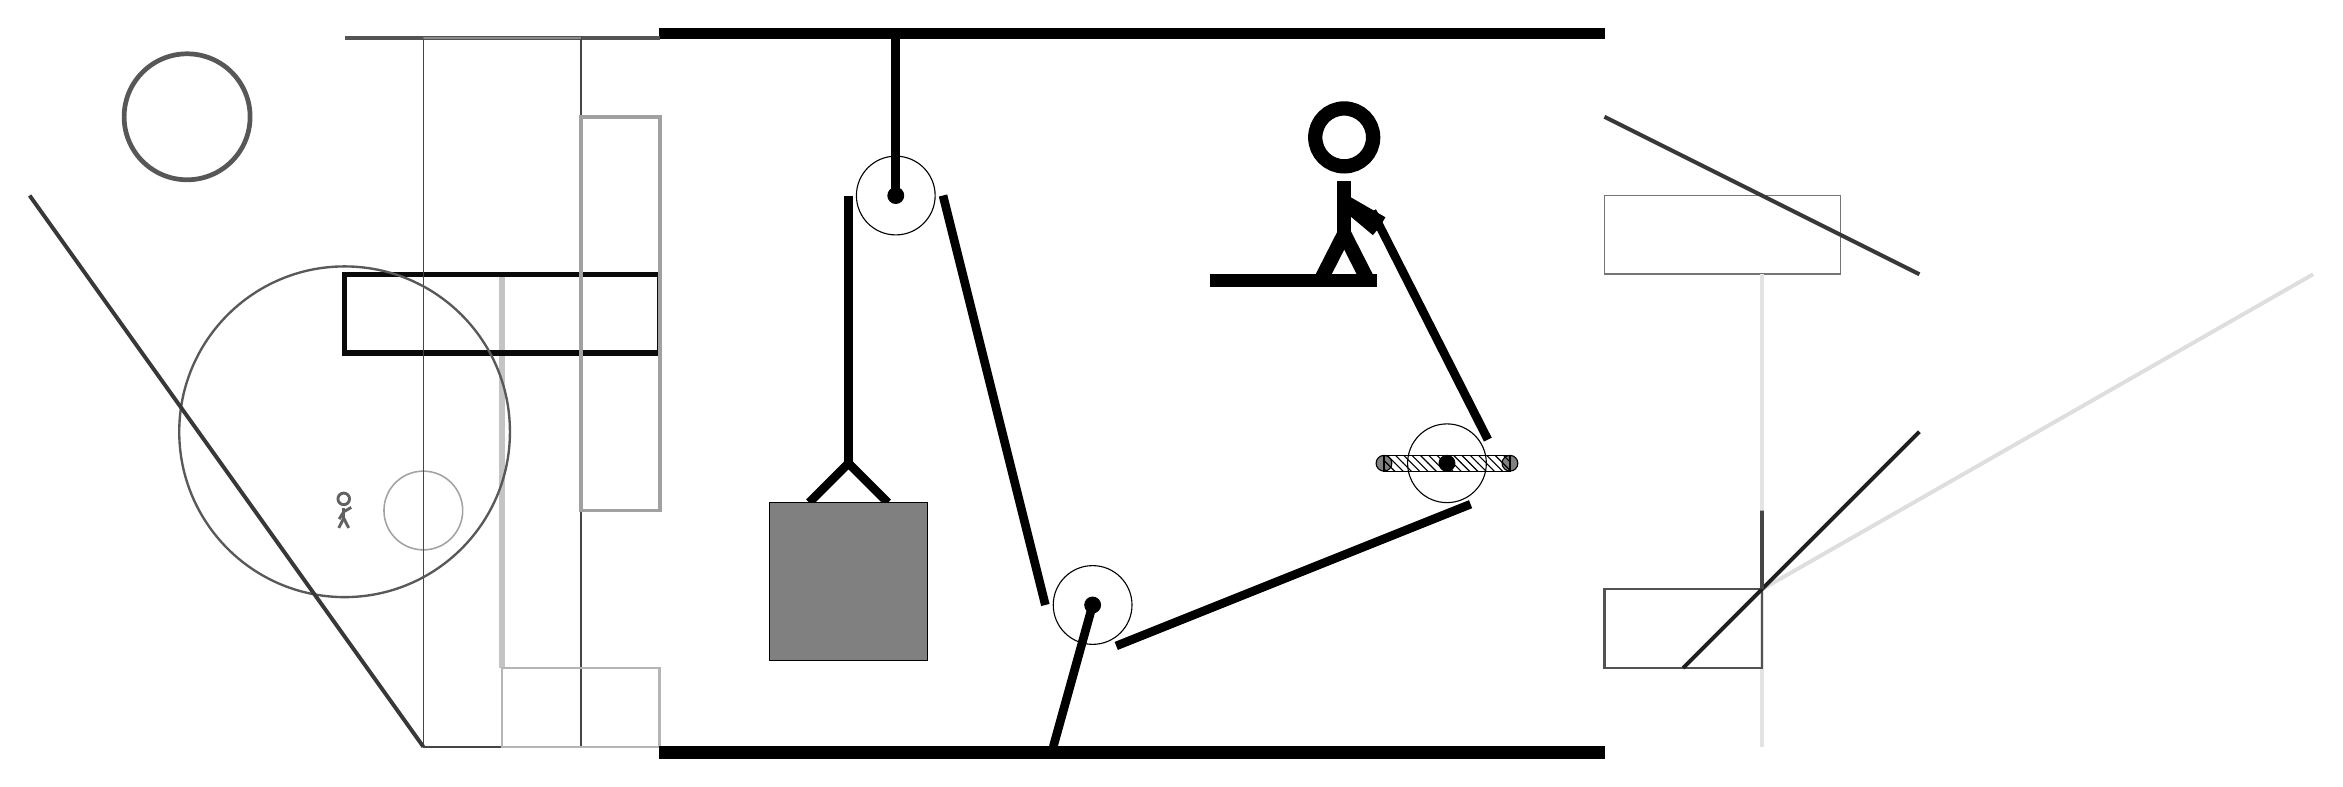
\begin{tikzpicture}
			%%%%% START %%%%%
			
			\draw[fill=black] (-2, 9) rectangle (10, 9.125);
			
			\draw (1, 7) circle (0.5);
			\draw[fill=black] (1, 7) circle (0.1);
			\draw[line width=1.1mm] (1, 9) -- (1, 7);
			
			\draw (3.5, 1.8) circle (0.5);
			\draw[fill=black] (3.5, 1.8) circle (0.1);
			\draw[line width=1.1mm] (3.5, 1.8) -- (3.0, 0);
			
			\draw[fill=white](8, 3.6) circle (0.5);
			\draw[fill=black] (8, 3.6) circle (0.1);
			\draw[fill=black!50] (8.8, 3.6) circle (0.1);
			\draw[fill=black!50] (7.2, 3.6) circle (0.1);
			\draw[pattern=north west lines, pattern color=black] (7.2, 3.7) rectangle (8.8, 3.5);
			
			\draw[line width=1.1mm](-0.1, 3.1) --  (0.4, 3.6) -- (0.9, 3.1);
			\draw[fill=black!50] (-0.6, 3.1) rectangle (1.4, 1.1);
			
			\draw[line width=0.5mm, color=black!67](-2, 9) -- (-6, 9);
			
			\draw [line width=0.2mm, color=black!36](-5, 3) circle (0.5);
			\draw[line width=0.2mm, color=black!54] (10, 7) rectangle (13, 6);
			\draw[line width=0.5mm, color=black!13](12, 2) -- (19, 6);
			\draw[line width=0.5mm, color=black!11](12, 0) -- (12, 6);
			
			\draw[line width=0.7mm, color=black!23] (-4, 1) rectangle (-4, 6);
			\draw[line width=0.3mm, color=black!68] (12, 2) rectangle (10, 1);
			\draw[line width=0.7mm, color=black!96] (-2, 5) rectangle (-6, 6);
			\node[line width=0.2mm, color=black!62] at (-6, 3) {\Strichmaxerl[2][58][30]};
			\draw[line width=0.2mm, color=black!73] (-3, 0) rectangle (-5, 9);
			
			\draw[line width=0.3mm, color=black!29] (-4, 0) rectangle (-2, 1);
			
			\draw [line width=0.3mm, color=black!65](-6, 4) circle (2.1);
			\draw [line width=0.6mm, color=black!68](14, 8) circle (0.0);
			
			\draw[line width=0.5mm, color=black!78](14, 6) -- (10, 8);
			\draw [line width=0.6mm, color=black!66](-8, 8) circle (0.8);
			\draw[line width=0.2mm, color=black!45] (-3, 9) rectangle (-5, 9);
			
			\draw[line width=0.5mm, color=black!88](11, 1) -- (14, 4);
			\draw[line width=0.5mm, color=black!37] (-3, 3) rectangle (-2, 8);
			\draw[line width=0.5mm, color=black!78](-5, 0) -- (-10, 7);
			\draw[line width=0.5mm, color=black!73] (12, 2) rectangle (12, 3);
			
			\draw[line width=1.1mm](0.4, 7) -- (0.4, 3.6);
			\centerarc[line width=1.1mm](1, 7)(180:0:0.6)
			\draw[line width=1.1mm](1.6, 7) -- (2.9, 1.8);
			\centerarc[line width=1.1mm](3.5, 1.8)(180:300:0.6);
			\draw[line width=1.1mm](3.8, 1.2804) -- (8.3, 3.0804);
			\centerarc[line width=1.1mm](8, 3.6)(300:390:0.6);
			\draw[line width=1.1mm](8.5196, 3.9) -- (7.05, 6.8);
			
			\node at (6.75, 7) {\Strichmaxerl[10][-220][-30]};
			\draw[fill=black] (5, 6) rectangle (7.1, 5.85);
			
			\draw[fill=black] (-2, 0) rectangle (10, -0.15);
			
			%%%%% END %%%%%
		\end{tikzpicture}
	\end{figure}	
\end{document}